\documentclass[14pt]{beamer}
\usepackage{colortbl}
\usepackage{tikz-qtree}

\title[GLAMR]{GLAMR: Graph Languages for Abstract Meaning Representations}
\date{2014 Aug 1}

% for drawing graphs
\usepackage{tikz,tikz-qtree}
%\usetikzlibrary{graphdrawing}
\usetikzlibrary{arrows}
\tikzstyle{internal}=[circle,draw=black,thick,inner sep=1mm]
\tikzstyle{internalnum}=[circle,draw=black,inner sep=0.5mm,font={\tiny}]
\tikzstyle{external}=[circle,draw,fill=black,inner sep=1mm]
\tikzstyle{externalnum}=[circle,draw,fill=black,inner sep=0.5mm,font={\color{white}\tiny}]
\tikzset{level distance=1cm,sibling distance=0.5cm}
\tikzset{edge/.style={draw,-latex}}
\tikzset{edge from parent/.style={edge,edge from parent path={(\tikzparentnode)--(\tikzchildnode)}}}
\tikzset{llabel/.style={auto=right,inner ysep=1pt,inner xsep=2pt}}
\tikzset{rlabel/.style={auto=left,inner ysep=1pt,inner xsep=2pt}}
\tikzset{every leaf node/.style={anchor=north}}
\newcommand{\sem}[1]{\strut\ensuremath{{\mathit{#1}'}}}
\newcommand{\semstate}[2]{\strut\ensuremath{{#2:\mathit{#1}'}}}

\begin{document}
\section{test}
\begin{frame}{Recognition}

\begin{center}
\begin{tikzpicture}
\node[anchor=east,name=g] at (-3,2) {Graph $G$};
\node[anchor=east,name=m] at (-3,-2) {Grammar $M$};
\node[draw,name=r,inner ysep=5mm] {Recognition};
\node[anchor=west,name=o] at (2,0) {$G \in \mathcal{L}(M)$?};
\draw[-latex,out=0,in=180] (g) to (r);
\draw[-latex,out=0,in=180]  (m) to (r);
\draw[-latex] (r) to (o);
\end{tikzpicture}
\end{center}

\end{frame}

\section{Synchronous Hyperedge Replacement Grammar Learning} % Xiaochang Peng, 10 minutes
\frame{\sectionpage}

\subsection{Definition}


\newbox\gbox

\begin{frame}{Learning HRG rules}
\global\setbox\gbox\hbox{%
\begin{minipage}{\hsize}
\begin{align*}
S &\rightarrow 
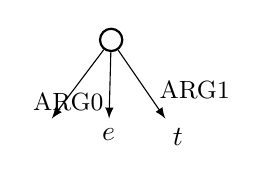
\begin{tikzpicture}[baseline=-1mm]
\Tree [.\node[internal]{}; \edge[llabel]node[name=m]{\small};$$ \edge[llabel,near end] node{\small ARG0}; $e$ \edge[rlabel,near end] node{\small ARG1}; $t$ ] 
\end{tikzpicture} &
S &\rightarrow 
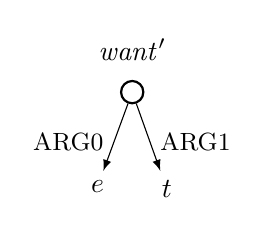
\begin{tikzpicture}[baseline=-1mm]
\Tree [.\node[internal,label=above:{\sem{want}}]{}; \edge[llabel,near end] node{\small ARG0}; $e$ \edge[rlabel,near end] node{\small ARG1}; $t$ ] 
\end{tikzpicture} &
e &\rightarrow 
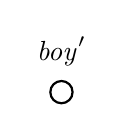
\begin{tikzpicture}[baseline=-1mm]\node[internal,label=above:{\sem{boy}}]{};\end{tikzpicture}
\\
t &\rightarrow 
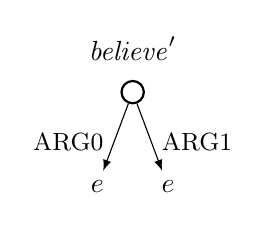
\begin{tikzpicture}[baseline=-1mm]
\Tree [.\node[internal,label=above:{\sem{believe}}]{}; \edge[llabel,near end] node{\small ARG0}; $e$ \edge[rlabel,near end] node{\small ARG1}; $e$ ] 
\end{tikzpicture} &
e &\rightarrow 
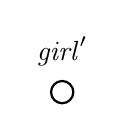
\begin{tikzpicture}[baseline=-1mm]\node[internal,label=above:{\sem{girl}}]{};\end{tikzpicture}
\end{align*}
\end{minipage}}

\copy\gbox

\end{frame}

\begin{frame}{Regular graph grammars}


\begin{tabular}{@{\hspace{-1cm}}cc}
\scalebox{0.5}{\copy\gbox}
&
%\begin{overlayarea}{10cm}{10cm}
\only<1>{$t$}%
\only<2>{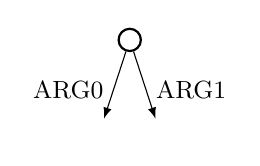
\begin{tikzpicture}[baseline=-1mm]
\Tree [.\node[internal]{}; \edge[llabel,near end] node{\small ARG0}; $$ \edge[rlabel,near end] node{\small ARG1}; $$ ] 
\end{tikzpicture}}%
\only<3>{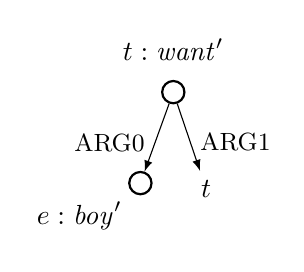
\begin{tikzpicture}[baseline=-1mm]
\Tree [.\node[internal,label=above:{\semstate{want}{t}}]{}; \edge[llabel,near end] node{\small ARG0}; \node[internal,label=below left:{\semstate{boy}{e}}]{}; \edge[rlabel,near end] node{\small ARG1}; $t$ ]
\end{tikzpicture}}%
\only<4>{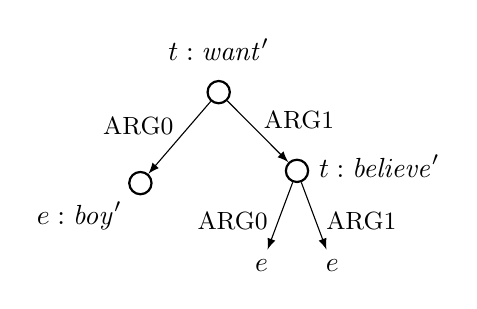
\begin{tikzpicture}[baseline=-1mm]
\Tree [.\node[internal,label=above:{\semstate{want}{t}}]{}; \edge[llabel] node{\small ARG0}; \node[internal,label=below left:{\semstate{boy}{e}}]{}; \edge[rlabel] node{\small ARG1}; [.\node[internal,label=right:{\semstate{believe}{t}}]{}; \edge[llabel,near end] node{\small ARG0}; $e$ \edge[rlabel,near end] node{\small ARG1}; $e$ ] ] 
\end{tikzpicture}}%
\only<5>{\hspace{-1cm}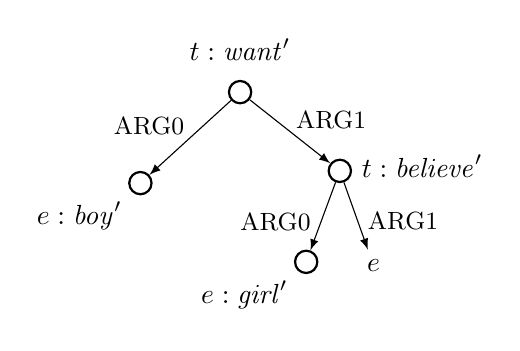
\begin{tikzpicture}[baseline=-1mm]
\Tree [.\node[internal,label=above:{\semstate{want}{t}}]{}; \edge[llabel] node{\small ARG0}; \node[internal,label=below left:{\semstate{boy}{e}}]{}; \edge[rlabel] node{\small ARG1}; [.\node[internal,label=right:{\semstate{believe}{t}}]{}; \edge[llabel,near end] node{\small ARG0}; \node[internal,label=below left:{\semstate{girl}{e}}]{}; \edge[rlabel,near end] node{\small ARG1}; $e$ ] ]
\end{tikzpicture}}%
\only<6>{\hspace{-1cm}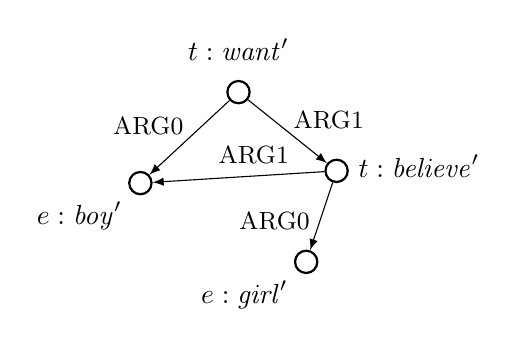
\begin{tikzpicture}[baseline=-1mm]
\Tree [.\node[internal,label=above:{\semstate{want}{t}}]{}; \edge[llabel] node{\small ARG0}; \node[internal,label=below left:{\semstate{boy}{e}},name=boy]{}; \edge[rlabel] node{\small ARG1}; [.\node[internal,label=right:{\semstate{believe}{t}},name=believe]{}; \edge[llabel,near end] node{\small ARG0}; \node[internal,label=below left:{\semstate{girl}{e}}]{}; \edge[draw=none]; \node{}; ] ]
\draw[edge] (believe) to node[auto=right,pos=0.15]{\small ARG1} (boy);
\end{tikzpicture}}%
\only<7>{\hspace{-1cm}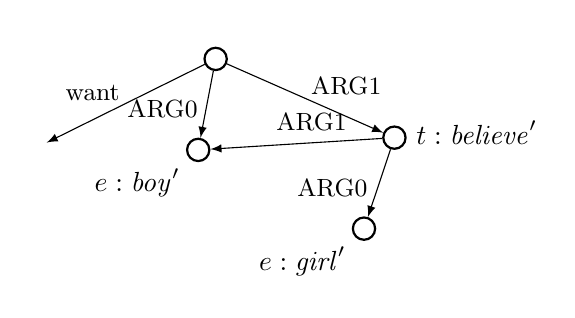
\begin{tikzpicture}[baseline=-1mm]
\Tree [.\node[internal,label=above:{}]{}; \edge[llabel] node{\small want};$$ \edge[llabel, near end] node{\small ARG0}; \node[internal,label=below left:{\semstate{boy}{e}},name=boy]{}; \edge[rlabel] node{\small ARG1}; [.\node[internal,label=right:{\semstate{believe}{t}},name=believe]{}; \edge[llabel,near end] node{\small ARG0}; \node[internal,label=below left:{\semstate{girl}{e}}]{}; \edge[draw=none]; \node{}; ] ]
\draw[edge] (believe) to node[auto=right,pos=0.15]{\small ARG1} (boy);
\end{tikzpicture}}%
%\end{overlayarea}
\end{tabular}
\\[1cm]
The boy wants the girl to believe him.

%\tikz \graph [tree layout, depth first spanning tree]
%{
%	1 --[bend right] {2, 3};
%};

\end{frame}




\end{document}